% Chapter 1
\documentclass[../main.tex]{subfiles}
%------------------------------------------------
\begin{document}
%------------------------------------------------
% Format for this section.
% - Introduce/explain why we want to cluster.
% - Explain two methods in literature (PCA Agne, Delaigle)
% - Examples of performance on simulated simple data.
% - Discuss Pros v cons.
% - Introduce/discuss Haar basis in more detail
% - Explain how to extract features using the Haar. DONE
% - Examples on surrogate data  DONE
% - Apply to bulk simulated data - explain clustering. 
% - Application to the real data.	
%   > Fit with/without trends. 
%   > Fit to Colin 1.
%   > Fit with Martin 4.
% - Discussion
%
% What data are we looking at. I.e how we get to intensity functions for an entire dataset. 
Previously we have shown how to obtain \ce{Ca^2+} spike sequences from fluorescence time course data of intracellular \ce{Ca^2+} concentration. We have utilised the \ce{Ca^2+} spike sequences to infer the parameters of our model --- the intensity function and ISI parameters. Crucially, the inferred intensity function describes the mean spiking rate of the cell. This can be seen in Figure \ref{fig:SoFar} (A), (B) and (C) for a single cell in a step change experiment (data kindly provided by M. Falcke). We threshold the time course data (A) to obtain a \ce{Ca^2+} spike sequence. We then use the \ce{Ca^2+} spike sequence (B) to obtain the posterior distribution for the intensity function. In Figure \ref{fig:SoFar} (C) we see the posterior mean (black line) with the 95\% confidence interval (grey region). The cell shown belongs to a dataset containing 13 other cells. Thus we can obtain the posterior distribution of the intensity function for each cell individually. In Figure \ref{fig:SoFar} (D) we plot the mean posterior intensity function for each cell in the dataset.  This plot shows the variability of how a cell reacts to the same stimulus. In this case we see that the mean spiking rate varies between $0$ and $0.03$. Furthermore, we see that most functions contain a peak in $[0,1000]$ and another in the region $[3400,4000]$. However, not all functions show the same behaviour, in particular the red line's `peaks' appear to last longer and its intensity tends to be higher than the other intensity functions.

 %Plot ofsoFar.  
     \begin{figure}[t!]
   \hrulefill
   \begin{center} 
    {\includegraphics[width = 0.95\linewidth]{SoFar.pdf} }
    \end{center}     
    \caption{An explanation of how we generate intensity functions (D) from experimental data. For a single cell we begin with a Fura-2 fluorescence intensity trace (A) --- the changes in the fluorescence of the \ce{Ca^2+} indicator is recored relative to its basal level ($\Delta F$) --- which is thresholded to calculate \ce{Ca^2+} spike times (B). The \ce{Ca^2+} spike times are used as an input into our model which returns the posterior distribution of the intensity function (C). The posterior distribution in (C) shows the mean (black line) with 95\% confidence interval (grey region).}
    \label{fig:SoFar}
    \hrulefill
    \end{figure}
    
% What are we doing and why is this important?
In this chapter we investigate how to partition intensity functions --- such as those in Figure \ref{fig:SoFar} (D) ---  into groups that have similar properties. We want to group the intensity functions as this will give insight into how cells respond to stimulus.
 Firstly, consider cells exposed to a constant stimulus. It is often assumed that after some initial transience \ce{Ca^2+} oscillations relax into a stationary regime. This means that the spiking rate converges to a constant. Many models have been developed with this assumption \cite{Skupin_2008, Skupin_2010}. However our model makes no such assumption on the mean spiking rate. This allows us to fit the mean \ce{Ca^2+} spike rate over the entire time course (not removing initial transients) and identify trends in this rate. With the inclusion of initial transients we can explore if each cell experiences a similar transient period. For example do we find that the transient period lasts the same length of time for all cells? In addition, what shape does the intensity take in the transient period? For example, the intensity could gradually decrease or oscillate as it converges to a constant. Moreover, do we find that the intensity converges at all? To fit models assuming the \ce{Ca^2+} times are stationary it is sometimes required to remove linear trends in the ISI, which is justified as fluorescent dyes used to record the \ce{Ca^2+} concentration acts as a \ce{Ca^2+} buffer \cite{Thurley_2014}. Thus, we may expect to find that the intensity decreases over time. If this is the case, do all cells show this decrease and is the amount the intensity decrease similar for each cell? If not, this could point to other mechanisms controlling the decreasing intensity such as negative feedback dynamics found in the cell. Thus, grouping the intensity functions inferred from constant stimulus experiments will test the assumption if a constant spike rate is biologically realistic. 
%Clustering also identifies cells which experience a similar  Furthermore, the features which we group the functions can give insight into the dynamics controlling the \ce{Ca^2+} concentration in cells. 

 Now consider cells challenged with a time-dependent stimulus. Do we find that a cell's intensity mirrors the applied stimulus, and does this happen for all cells? Furthermore, this analysis can be applied to cells challenged with agonist time courses that mimic physiological conditions in vivo. Thus, allowing us to investigate cell's spiking rate from a realistic environment.  

 
 In the above considerations  each cell is challenged with the same stimulus. However, we can also cluster intensities where groups of cells are exposed to different stimuli. In this case, if the clusters can distinguish between different stimuli this will give insight into how the stimuli affect the \ce{Ca^2+} concentration. Furthermore, if we can match cells to their stimulus then we can analysis populations of cells and find which cells in the population receive similar stimuli, which in turn can aid understanding of how signals transmit through populations of cells.

% What is clustering and how do we do it in simple case.
The challenge of grouping together objects is known as clustering. The aim of clustering is to group together objects such that objects in the same group are more similar than objects in other groups \cite{Friedman2001}. For example points in two dimension are similar if they are close together. As such, the clusters generated depend on the definition of similarity and initial assumptions \cite{Estivill_Castro_2002}. Rather than considering the intensity functions let us begin by first simplifying our problem; represent each function by its mean and variance, shown as the points in Figure \ref{fig:k_means}. Now our problem involves partitioning these points into groups, depending on the proximity of the points. One method to cluster these points is to use k-means clustering \cite{Arthur_2007}. This involves finding centers (crosses in Figure \ref{fig:k_means}) ---  where each point belongs to their nearest center --- optimised such that the distance of all points to their corresponding center is minimised. Thus, Figure \ref{fig:k_means} shows how the points are clustered using this approach with three clusters. Choosing the number of clusters is another problem, for k-means we would compare the total width of all the clusters. For example, in Figure \ref{fig:k_means} the total distance of points from their center is $ 1.26$, whereas with two clusters the total distance would be $2.82$. In addition to k-means there exists other clustering methods such as: mean shift \cite{Comaniciu_2002}, DSBSCAN \cite{Ester_1996} or spectral clustering \cite{Ng_2001}. Each of these methods are easy to apply on two-dimensional data, but not to functions. By using only the mean and variance of our intensity functions we lose information, and most importantly how the intensity varies over time.  
%Plot of k-means example.  
     \begin{figure}[t!]
   \hrulefill
   \begin{center} 
   {\includegraphics[width = 0.8\linewidth]{Ex_k_means.pdf} }
    \end{center}     
    \caption{Example of clustering using k-means with 3 clusters. Each point on the graph corresponds to a single intensity function. Red/black/green corresponds to which cluster the intensity function belongs. The crosses correspond to the center of each cluster.}
    \label{fig:k_means}
    \hrulefill
    \end{figure}
    

 %For example, the functions shown in Figure \ref{fig:SoFar} (D) could be clustered according to the shape, intensity or spatial position.
%Extension of clustering on our dataset. How do we want to cluster the functions/
 We mentioned previously that we want to cluster objects that have similar properties, but what does this mean for functions? Consider once again the functions in Figure \ref{fig:SoFar} (D). In this case we could say functions are similar if their intensities remain close between $0$s and $6860$s, or if they have the same properties, such as a peak in intensity around 3500s. Recall that  the same type of cell exposed with the same stimulus experiences large cell-to-cell variability. For example HEK293 cells stimulated with $10\mu\mathrm{M}$ carbachol were found to have between $9$ and $87$ \ce{Ca^2+} spikes over $3000$s. Hence, the mean firing rate varies widely from cell to cell. With this in mind, we aim to cluster our intensity functions via their features, rather than the absolute rate. By features, we refer to properties such as increasing and decreasing regions and peaks/troughs in the intensity. Any region where a peak occurs --- an initial increase in rate followed by a decrease --- we shall refer to as a bump.   For example, suppose we have 3 intensity functions (black, red and blue lines in Figure \ref{fig:Similar})  from an experiment that lasts $3000$s with mean spiking rate of $1$, $1$ and $0.5$ respectively. Suppose further that only the first and last functions increase in the region $[0,1000]$ and have a bump in the region $[2000,3000]$,  while the second function is constant. Although the first and third functions (black and blue lines) have significantly different mean rates, we may want to cluster these functions in the same group since they have the same shape. Whereas, even though the first two functions (black and red lines) have the same mean firing rate, due to their differing features we do not group these together. 

 %Plot of clustering methodology. 
     \begin{figure}[t!]
   \hrulefill
   \begin{center} 
    {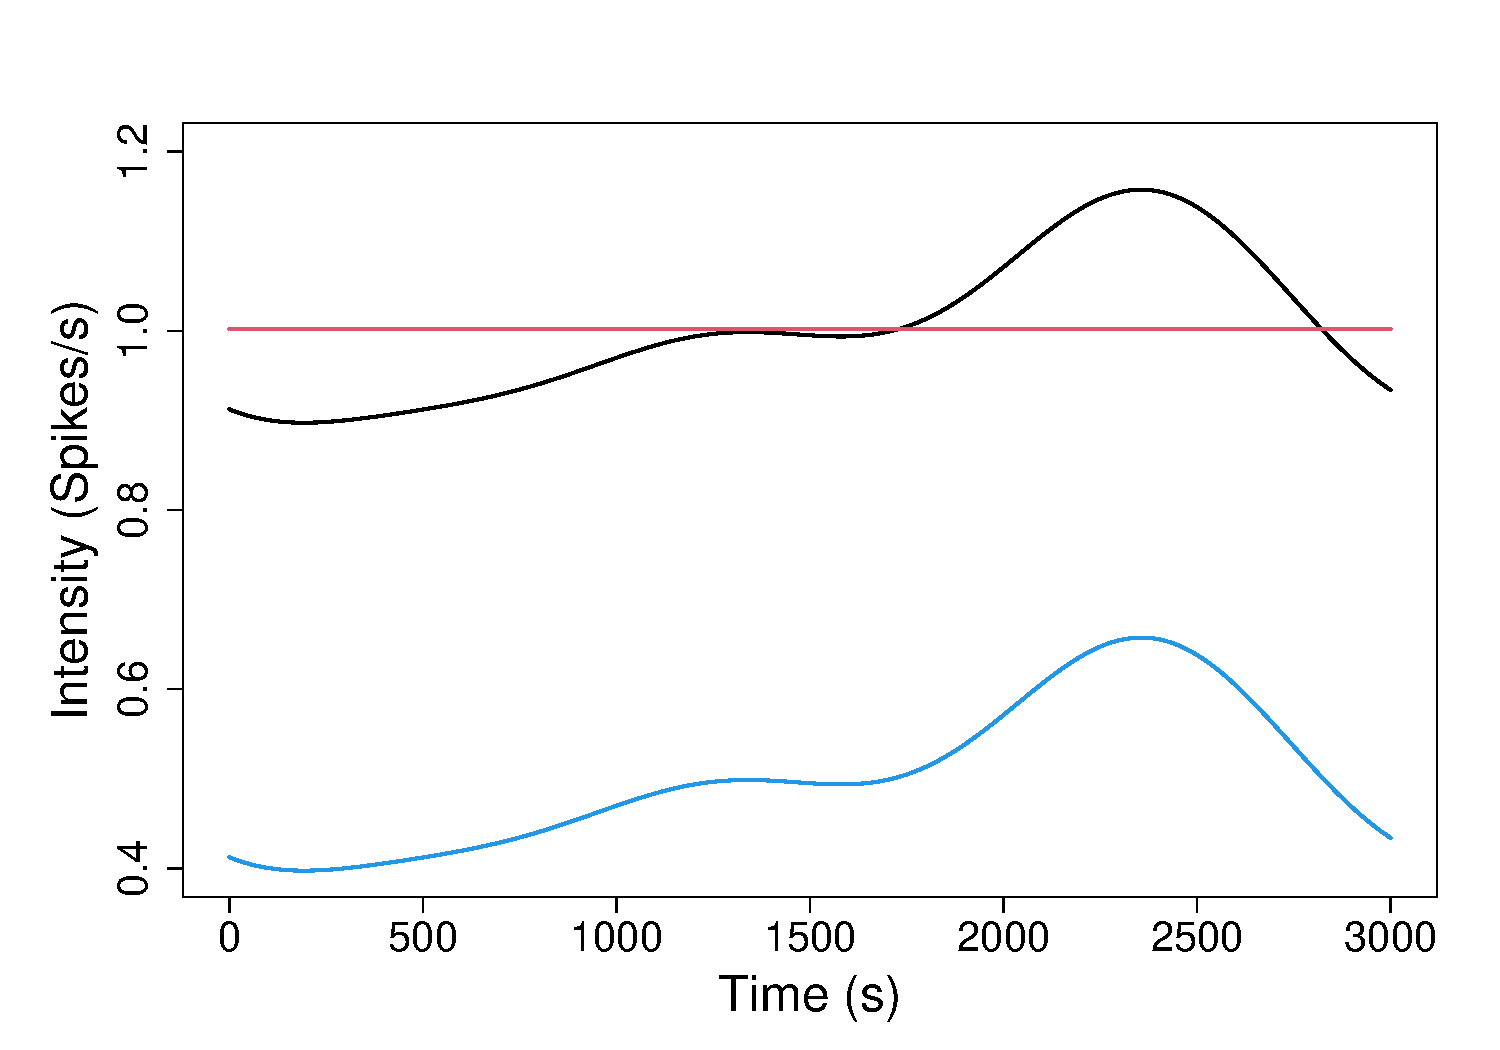
\includegraphics[width = 0.8\linewidth]{Similar.pdf} }
    \end{center}     
    \caption{Example of clustering methodology applied to three functions. The black and blue lines are grouped together as they have similar shape. Whereas, although the red and black lines have a similar intensity they will not be grouped together as they have different shapes.}
    \label{fig:Similar}
    \hrulefill
    \end{figure}

% Metods in literature to cluster functions.
We now require a method that clusters functions with respect to such features. 
Since functions have infinite dimensions we cannot directly apply the clustering methods mentioned previously. One way to mitigate this challenge is to decompose the functions into a finite number of variables where we can use standard clustering methods. Tilunaite et al \cite{Tilunaite_2017} did exactly this to intensity functions calculated from \ce{Ca^2+} oscillations. They decomposed each  function into its three leading principal components, using principal component analysis (PCA). They then clustered the components using k-means, mean shift, DBSCAN and spectral clustering. They found that the clustering methods could not detect one unique cluster structure. Hence, they applied k-means for their analysis due to its speed and simplicity. More recently, Delaigle et al \cite{Delaigle_2019} developed a method specifically designed to cluster functions. Their method consists of applying a weighted k-means on projections of each function onto a space of finite dimension $p$, where rather than project onto a predetermined basis ---  such as a principal component basis --- the projection is chosen to optimise clustering performance. In practice this is done by first approximating each function via the Haar basis and projecting the coefficients into a space of $p$ dimensions in a manner to optimise clustering. This method has been shown to cluster asymptotically perfectly in some cases. This means if we have two populations in the dataset which differ in their means, then as the sample size increases the proportion of data from one population belonging to the same cluster tends to one.  

  %Plot of Delaigle/Tilunite performing badly. 
     \begin{figure}[ht!]
   \hrulefill
   \begin{center} 
  \subfloat[]{{\includegraphics[width = 0.45\linewidth]{PCA_Bad.pdf} }} \quad
      \subfloat[]{{\includegraphics[width = 0.45\linewidth]{Delaigle_Bad.pdf} }}\\ 
    \end{center}     
    \caption{Clustering a dataset containing constant functions and functions with a single bump. In (A) we cluster using the method in Tilunaite and (B) Delaigle.}
    \label{fig:FitBad}
    \hrulefill
    \end{figure}

% Methods in liturature don't perform how we want.
 We now test the methods proposed by Titunaite \cite{Tilunaite_2017} and Delaigle \cite{Delaigle_2019} on surrogate data with attributes similar to those that intensity functions inferred from experimental data contain. The performance of these methods on these datasets can be viewed in Appendix $\text{}$A1. We found that both methods perform well in some situations but not others. In particular, both methods fail to cluster a dataset containing constant functions and functions with varying bump placements. In Figure \ref{fig:FitBad} we show the results of clustering for this dataset where the two clusters are represented by the colour (red/black) of the lines. Figure \ref{fig:FitBad} (A) shows that the method proposed by Titunaite clusters functions that have a bump around 1000s, whilst the remaining functions with bumps are grouped with the constant functions. Figure \ref{fig:FitBad} (B) shows that the method proposed by Delaigle clusters 5 bumps centered around 500s with the constant functions. Thus, neither method managed to group all the functions with bumps together. 
 
 %Number of clusters challenge.
 Another challenge in clustering is choosing the number of clusters. Some methods automatically choose the number of clusters such as DBSCAN and mean shift. Titunaite et al \cite{Tilunaite_2017} set the number of clusters in their case to 5, having noted that differing methods found different number of clusters.   
 
 % What we do.
 In light of the above, we have developed our own method, specifically designed to decompose functions into their features which we can then cluster. We begin by describing each function by the number and type of features it has. For example a function could be described by decreasing in $[0,100]$ and a bump in the region $[1000,1500]$. Furthermore, we will provide each feature with a magnitude which describes how large the feature is, which can be used to detect the important features. The benefit of this approach is that it prioritises the shape of the features over the exact value of the function. 
 The clustering is performed by comparing the features of individual functions and is done at the user's discretion, rather than using a clustering algorithm. The advantage of this method is it allows flexability in the clustering and allows the user to choose the type of clusters. For example we	 may be interested in the interval $[200,500]$ and we can cluster on the behaviour in this interval. In a different situation we may be interested in the total number of bumps over the entire function, which can then be clustered accordingly. 
 
 In the following sections we explain how to extract features of functions by utilising the Haar basis and how to find a feature's magnitude. We then explain how to cluster on an example dataset, before applying our method to data from HEK293 cells stimulated with carbachol. 

%%%%%%%%%%%%%%%%%%%%%%%%%%%%%%%%%%%%%%%%%%%%%%
\section{The Haar basis}
%Why we using the Haar basis.
The Haar basis is a sequence of square-like functions that forms an orthonormal basis on $L^2[\mathbb{R}]$ --- the space of square-integrable functions on $\mathbb{R}$ . Originally, the basis was put forward by Alfred Haar in $1909$ as an example of an orthonormal basis on $[0,1]$ \cite{Haar_1910}. The basis was the first known example of a wavelet --- a series of mathematical functions that cuts up data into different frequency components --- although this concept was only invented in 1982, 73 years after Alfred Haar first constructed the basis \cite{Debnath_2003}.  
 
We were motivated to use the Haar basis because it was used by Delaigle et al \cite{Delaigle_2019} in their approach for clustering functions. They found that the Haar basis captures both local and global trends without requiring a large number of bases. We also find that the formation of the basis is well suited to finding locations of features, as described in the next section. 

%There exists other orthonormal bases such as: principal component basis, Fourier basis, etc \cite{}. However, we found the Haar basis 

% Definition of the Haar basis, and bases on the interval[0,T].
 Since we are only considering functions on bounded intervals, we derive the Haar basis on the interval $[0,T]$ equipped with the $L^2$-inner product $\langle f,g \rangle = \int^T_0 fg \text{ }  dt$ for $f,g \in L^2\left( \left[0,T \right] \right)$. The basis consists of functions formed by scaling and shifting the Haar mother function, 
\begin{equation*}
\psi(t) =
\begin{cases}
	1 & 0 \leq t < 0.5,\\
	-1 & 0.5 \leq t <1,\\
	0 & \text{otherwise,}\\
\end{cases} 	
\end{equation*}

%Plot of the first 8 Haar basis vectors. 
  \begin{figure}[ht!]
   \hrulefill
   \begin{center} 
    \subfloat[$h_1$]{{\includegraphics[width = 0.42\linewidth]{HaarBasis1.pdf} }} \quad
      \subfloat[$h_2$]{{\includegraphics[width = 0.42\linewidth]{HaarBasis2.pdf} }}\\ 
      
         \subfloat[$h_3$]{{\includegraphics[width = 0.42\linewidth]{HaarBasis3.pdf} }} \quad
      \subfloat[$h_4$]{{\includegraphics[width = 0.42\linewidth]{HaarBasis4.pdf} }}\\
       
         \subfloat[$h_5$]{{\includegraphics[width = 0.42\linewidth]{HaarBasis5.pdf} }} \quad
      \subfloat[$h_6$]{{\includegraphics[width = 0.42\linewidth]{HaarBasis6.pdf} }} \\
     
       \subfloat[$h_7$]{{\includegraphics[width =0.42\linewidth]{HaarBasis7.pdf} }} \quad
      \subfloat[$h_8$]{{\includegraphics[width = 0.42\linewidth]{HaarBasis8.pdf} }}
    \end{center}     
    \caption{The first 8 Haar bases on the interval $[0,20]$.}
    \label{fig:HaarBasis}
    \hrulefill
    \end{figure}


and a constant function \cite{Haar_1910}.  Since we are forming an orthonormal basis we require the bases to be normalised and orthogonal. This means that for bases $h_i$ and $h_j$ we require $\langle h_i, h_j \rangle = \delta_{i,j}$, where $\delta_{i,j}$ represents the Kronecker delta. The bases will consist of stretching the Haar mother such that each base is zero everywhere except for a region of length $T/2^a$ for some $a \in \mathbb{N}$. Thus, to satisfy the normality condition  each function will be scaled by a factor of $\sqrt{2^{a}/ T}$.

 We will briefly explain how the first 8 bases are determined.  The first base $h_1$ is defined as the constant function taking value $1/ \sqrt T$. The second base $h_2$ is the Haar mother function stretched to take non-zero values on $[0,T]$ and scaled by $1/ \sqrt T$, $h_2 = (1/ \sqrt T)\psi(t/T)$. By definition this is a step function with  height $1/ \sqrt T$ in $[0,T/2]$ and $-1/ \sqrt T$ in $[T/2,T]$. The next two bases are $h_3 = \sqrt{2/T}\psi(2t/T)$ and $h_4 = \sqrt{2/T}\psi((2t-T)/T)$. These are scaled versions of the Haar mother function taking non-zero values only the intervals $[0,T/2]$ and $[T/2,T]$ respectively. The next 4 bases are created in the same manner by splitting the function into 4 equal regions $h_5 = (2/ \sqrt T)\psi(4t/T)$, $h_6 = (2/ \sqrt T)\psi((4t-T)/T)$, $h_7 = (2/ \sqrt T)\psi((4t-2T)/T)$ and $h_8 = (2/ \sqrt T)\psi((4t-3T)/T)$. The graphs of these 8 functions are shown in Figure \ref{fig:HaarBasis}, where $T$ was taken to be $20$. From these graphs we can visualise the orthogonality of the bases. Consider two bases $h_i$ and $h_j$. If the non-zero regions of the two bases do not overlap --- for example $h_4$ and $h_5$ in Figures \ref{fig:HaarBasis} (D) and (E) --- then their product $h_ih_j = 0$. Otherwise, if the bases do overlap the region that is non-zero in their product is just a multiple of the finer base. This can be seen in Figures \ref{fig:HaarBasis} (C) and (E) for bases $h_3$ and $h_5$, where the product of these two functions is a multiple of $h_5$. By construction $\int^T_0 h_i dt = 0$ for $i>1$, hence if $h_i$ and $h_j$ do overlap with $h_j$ finer than $h_i$ we get $\langle h_i,h_j \rangle = \int^T_0 h_i h_j dt = \int^T_0 C h_j dt = 0$, for some constant $C$.
 
    From this procedure notice that we generate the bases in levels, starting with $\{h_1\}$, then $\{h_2\}$, $\{h_3,h_4\}$, $\{h_5,h_6,h_7,h_8\}$ and so on. We label these levels 0, 1, 2 and 3 respectively. From Figure \ref{fig:HaarBasis} we see that each level $k$ consists of breaking the space into $l = 2^{k-1}$ equal regions. Consider the $k$th level, of which we generate $l$ bases $g_{1}, \dots, g_{l}$. Each base $g_i$ only takes non-zero values in a region of length $T/l$; for $g_1$ this region is $[0,T/l]$, for $g_2$ it is $[T/l,2T/l]$ and so forth. The non-zero region consists of a scaled version of the Haar mother function, where the first half of this region takes the value $\sqrt{l/ T}$ and the second half has value $-\sqrt{l/ T}$. More precisely we get 

$$g_{i} = \sqrt{\frac{l}{ T}}\psi \left( \frac{lt-(i-1)T}{T} \right).$$

In respect to the Haar basis the bases from the $k$th level corresponds to the bases $h_{l+1}, \dots, h_{2^k}$. In other words $h_{l+i} = g_{i}$. Since the sequence of Haar bases $\{h_i\}_{i=1}^{\infty}$ forms an orthonormal basis in $[0,T]$, any function $f(t)$ can be expressed as 
$$
f(t) = \sum^{\infty}_{i=1}  \alpha_{i} h_i,
$$
where $\alpha_i$ is the coefficient of the Haar base $h_i$, for $i \in \mathbb{N}.$

%General how do we calculate the coefficents of the bases?
Naturally, this poses the question: given a function $f(t)$ how do we calculate the Haar coefficients? Since our basis is orthonormal we can calculate the coefficient $\alpha_j$ of the base $h_j$ by considering the inner product of $f$ and the base $h_j$ 

\begin{align*}
\langle f,h_j\rangle &= \sum^\infty_{i=1} \alpha_i \langle h_i,h_j\rangle, \\
&= \sum^\infty_{i=1} \alpha_i \delta_{i,j}, \\
&= \alpha_j.
 \end{align*}
 
 However, in practice the functions we consider are discretised. In particular, we have the function of interest $\mathbf{f} = (f_0,\dots f_N)$ and discretised bases $\mathbf{h_j} = ((h_j)_0, \dots (h_j)_N)$ for $j \in \mathbb{N}$, where $f_k = f(kT/N)$, $(h_j)_k = h_j(kT/N)$, and $N$ large. In this case we choose to find the coefficient for the $j$th base $\alpha_j$ by
 \begin{align*}
\alpha_i &= \langle f,h_j\rangle, \\
&= \int^T_0 f(t)h_j(t) dt, \\
&\approx \sum^N_{k=0} \frac{T}{N}f_k (h_j)_k, \\
&= \frac{T}{N}\sum^N_{k=0} f_k (h_j)_k.
 \end{align*}
Other numerical integration method exists, for example using a  trapezoid rule or Simpson's rule. However, with $N$ large we found our method to be sufficient. 


%General Approximating function via Haar basis.
We want to approximate $f$ by calculating the coefficients for the first $q = 2^a$ Haar bases for some $a \in \mathbb{N}$. Rather than calculate each base individually using the formula above, we can calculate the bases by using matrices. To calculate the coefficients $\bm{\alpha} = (\alpha_1, \dots, \alpha_q)$ we first combine the discretised Haar bases into a basis matrix $\mathbf{B}$ --- of dimension $(N+1) \times q$ ---  where the $i$th column of $\mathbf{B}$ is $\mathbf{h_i}$. We then calculate the Haar coefficients by $\bm{\alpha} = (T/N) \mathbf{f}  \times \mathbf{B}$, which is analogous to the computation above. 

We can visual the Haar approximation compared to the original function by  computing $\mathbf{f_{\mathrm{approx}}} = \sum^q_{k=1} \alpha_k \mathbf{h_k} = \bm{\alpha} \times \mathbf{B}^T$.

%Consider the function $f$ defined on the interval $[0,T]$. We want to approximate $f$ by considering the first $q$ Haar bases. $q$ must be a power of 2 to allow for the largest level to span the entire function. Thus, we need to calculate the coefficients $\alpha_1, \dots \alpha_q$ of the Haar bases. We begin by discretising time into $N+1$ steps $\mathbf{t} = \{t_i\}^N_{i=0}$ where $t_i = iT/N$. Then express $f$ and $h_i$ for $i \in \{1, \dots, q \}$ as vectors $\mathbf{f} = (f_0,\dots f_N)$ and $\mathbf{h_i} = ((h_i)_0, \dots (h_i)_N)$, where $f_j = f(t_j)$ and $(h_i)_j = h_i(t_j)$ for $j = 0, 1, \dots, N$. Combine the discretised Haar bases into a basis matrix $\mathbf{B}$ - of dimension $(N+1) \times q$ -  where the $i$th column of $\mathbf{B}$ is $\mathbf{h_i}$.  We calculate the Haar coefficients $\bm{\alpha} = (\alpha_1,\dots, \alpha_q)$ by $\bm{\alpha} = \mathbf{B} \times \mathbf{f}^T /(N+1)$. To visualise the approximation compared to the original function, we can convert the Haar representation back to a function $\mathbf{f}_{\mathrm{approx}}$ defined on the grid $\mathbf{t}$. This is done by multiplying the coefficients by the transpose of the basis matrix,  $\mathbf{f}_{\mathrm{approx}} = \bm{\alpha} \times \mathbf{B}^T$. 
 
%Example of approximating a function using Haar basis. 
Let $f$ be a draw from a GP on the interval $[0,20]$ with length scale $3$ and step size $0.01$, shown as the black line in Figure \ref{fig:HaarApprox}. We then approximate $f$ by decomposing it into $32$ Haar bases. The coefficients of the first $16$ Haar bases can be seen in Table \ref{table:HaarCoef}.

\begin{table}[h!]
  \begin{center}
    %\caption{Haar decomposition of $f$ a draw form a GP.}
    \label{table:Haar}
    \begin{tabular}{|c|l|l|l|l|l|l|l|l|}
    \hline
      \textbf{Base} & $h_{1}$ & $h_{2}$ & $h_{3}$  & $h_{4}$ & $h_{5}$ & $h_{6}$ & $h_{7}$ & $h_{8}$ \\ 
      \hline
     $f$ &-0.39 & -5.54 & 2.94 & -1.14 & 3.23 & -2.76 & -0.03 & -0.34  \\ \hline
     \hline
 \textbf{Base} & $h_{9}$ & $h_{10}$ & $h_{11}$  & $h_{12}$ & $h_{13}$ & $h_{14}$ & $h_{15}$ & $h_{16}$ \\ \hline
 	 $f$ & 0.68 & 1.39& -0.32& -1.26& -0.13& -0.08& -0.25& -0.03  \\ \hline
    \end{tabular}
    \caption{The coefficients of the Haar bases for function $f$ drawn from a GP shown in Figure \ref{fig:HaarApprox}. }
    \label{table:HaarCoef}
  \end{center}
\end{table} 

 %Plot of function and haar basis approximations.  
     \begin{figure}[t!]
   \hrulefill
   \begin{center} 
    {\includegraphics[width = 0.8\linewidth]{Ex_Haar.pdf} }
    \end{center}     
    \caption{Approximating a function via the Haar basis. The function (black line) is approximated by using 2 (red), 8 (orange) and 32 (blue) Haar bases.}
    \label{fig:HaarApprox}
    \hrulefill
    \end{figure}
 
 In Figure \ref{fig:HaarApprox}, we plot the true function (black line) along with the Haar approximation for $q = 2,8$ and $32$ (red, orange and blue lines respectively). We see that by increasing $q$ the approximation improves. Note that where the Haar approximation is constant, this equals the mean of $f$ in this region.

%%%%%%% Section of Getting the features
\section{Extracting features}
We will now explain how to use the Haar basis to extract features from a function. We begin by expressing the function $f$, defined in the interval $[0,T]$, in terms of a Haar basis with $q$ bases

$$
f \approx \alpha_1 h_1 + \dots + \alpha_{q} h_q, 
$$

where for $i = 1, \dots , q$ the $\alpha_i$ are the coefficients of the Haar bases $h_i$. The advantage of the Haar basis is that the sign of the coefficient can inform us whether the function is increasing or decreasing in the corresponding interval.
% Assuming that the function is monotone in the interval.

For example consider the base $h_7$, which is shown in  Figure \ref{fig:HaarBasis} (G) for $T=20$. We see that the base is zero everywhere except for the interval $[T/2, 3T/4]$. In this interval $h_{7}$ is positive in $[T/2, 5T/8]$ and negative in $[5T/8, 3T/4]$. Thus, if $\alpha_7 >0$ then $\alpha_7 h_7$ would have the same shape as $h_7$ and it appears that the function would be decreasing in $[T/2, 3T/4]$. Whereas, if $\alpha_7 < 0$ then $\alpha_7 h_7$ is similar in shape to the reflection of $h_7$ in the x-axis and is negative in $[T/2, 5T/8]$ and positive in $[5T/8, 3T/4]$. This implies that the function is increasing in $[T/2, 3T/4]$. It is important to note that this is true only if the function does not vary too much in these intervals. For example consider the approximation with two Haar bases (red line) in Figure \ref{fig:HaarApprox}. By the above reasoning we would say the function is increasing in $[0,20]$, which does not capture how the function truly varies in this region. Hence, we will only consider the bases on the finest intervals because the function will vary less on those intervals. 

 %For example suppose $\alpha_{7} = 1$, then $\alpha_7 h_7 = h_7$ and this is exactly the function shown in Figure \ref{fig:HaarBasis} (G) --- if $T=20$. We see that the base is $0$ everywhere except for the interval $[T/2, 3T/4]$. In this interval $h_{7}$ is positive in $[T/2, 5T/8]$ and negative in $[5T/8, 3T/4]$. Thus, multiplying by a positive coefficient maintains the sign of the function in these intervals. This means $f$ is decreasing in this interval.  However, if  $\alpha_{7} = -1$ then $\alpha_{7}h_{7}$ is negative in $[T/2, 5T/8]$ and positive in $[5T/8, 3T/4]$. This can be visualised by reflecting Figure \ref{fig:HaarBasis} (G) in the $x$-axis. Thus $f$ is increasing in the interval.

We build on this idea to calculate the features of functions. The method is explained below in 5 steps.

%Suppose we a given a function $f$ that we want to extract features from, decreasing/increasing trends or local bumps in value. To do this we want to decompose the function into a Haar basis, and use the coefficients of the Haar bases to calculate the features. We describe the method below, where we set the number of bases considered to $q$ (multiple of 2). Thus by matrix multiplication we can approximate $f$ by

%where the $\alpha_i$ are the coefficients of the Haar basis vectors $h_i$.

{\bf Step 1: Consider the appropriate bases.} We have $q$ bases and each base informs us on the behaviour of the function in a different interval. Recall that $q$ must be a power of 2 and contains $x$ levels. Thus we consider only bases which inform us of details on the smallest intervals, i.e the bases in the $x$th level. The $x$th level corresponds to the final $p = q/2$ bases. Thus, set $\mathbb{B} = \{p+1, \dots, q\}$ the index of the bases to be considered. For example if $q=16$, we consider the last 8 bases and set $\mathbb{B} = \{9, 10, \dots, 16\}$.
 %Suppose that $q=16$, in this case the last 8 basis functions contains the information about the function in the finest intervals. For example $h_9$ is only non-zero in the interval $[0,0.125]$, similarly  $h_{10}$ is non zero in the interval $[0.125,0.25]$, and so on. 	As such these intervals may not inform on the size of features by will give an indication on their positions. Thus we only consider the last $q/2$ coefficients. Set $B = \{q/2+1, \dots , q \}$ to be the bases considered and $ A = \{\alpha_{q/2+1} , \dots , \alpha_q \}$ the coefficients of these bases.

{\bf Step 2: Find the important bases.} We need to decide which of the appropriate bases informs us on potential features. For a base to contribute to a feature we need the function to be significantly increasing or decreasing in the corresponding interval. An alternative view is that we need to remove the bases whose intervals remain almost flat, as this will not lead to a feature. Thus, we choose a threshold $\sigma_\mathrm{thres}$ such that we remove index $i$ from $\mathbb{B}$ if $|\alpha_i| < \sigma_\mathrm{thres}$.
 
 Choosing $\sigma_\mathrm{thres}$ can be a difficult task. The coefficients of the haar bases scales with the function's range. For example consider a new function $g = 10f$ and approximate $g$ with $q$ Haar bases giving $g \approx \sum^q_{i=1} \beta_i h_i$. Since $g$ is just a scaled version of $f$ we get $\beta_i = 10\alpha_i$ for all $i$. Hence the threshold value for function $f$ may not be appropriate for $g$. One approach to avoid this issue would be to scale the functions to a similar range before assessing features. However, this could cause insignificant features to become enhanced. Another issue arises from the choice of $q$. The larger we take $q$ the smaller the coefficients are due to the factor of 2 in the definition of the bases. With the above taken into account, we find that the threshold should depend on the range $\Delta$ and the number of bases $q$. Thus, we often take $\sigma_\mathrm{thres} = \Delta/10q $, which performed well on simulated data, with $q$ either 16 or 32. Note that this would lead to different thresholds been applied to different functions. In some cases, it may be preferable to threshold the functions with the same value for consistency.

 %For example suppose $\mathbb{A} = \{-0.05,-0.8,0.65,0.08\}$ and $\mathbb{B} = \{12,13,14,15\}$, and we choose $\sigma_\mathrm{thres} = 0.1$. Applying the threshold gives updated values  $\mathbb{A} = \{-0.8,0.65\}$ and $\mathbb{B} = \{13,14\}$.


 {\bf Step 3: Check for peaks.} In step 2 we removed bases that do not correspond to a significant increase or decrease. However, a flat interval could be interpreted as a peak of a bump, which is a feature we want to extract. To include a peak the function must be increasing prior to the peak and decreasing afterwards. Thus, to check whether we need to add a base back into $\mathbb{B}$ we require the prior base's coefficient to have negative value (an increase before) and the base after to have positive value (decrease afterwards). For example suppose base $i$ was removed from $\mathbb{B}$ after thresholding. If $\alpha_{i-1} < - \sigma_\mathrm{thres}$ and $\alpha_{i+1} > \sigma_\mathrm{thres}$ then we add $i$ into the set $B$.
 
 {\bf Step 4: Split $\mathbb{B}$ into groups.} Next we split $\mathbb{B}$ into groups that correspond to different features. This is done by partitioning the set $\mathbb{B}$ into sets of consecutive bases, $B_1, B_2, \dots, B_n$. For example, suppose $\mathbb{B} = \{9,10,13,14,16\}$, then we split into 3 groups $B_1 = \{9,10\}$, $B_2 = \{13,14\}$, and $B_3 = \{16\}$.    
 
{\bf Step 5: Determine the features.} We now look at each of the groups $B_1, B_2, \dots, B_n$ individually. Consider the group $B_i$. If the group only contains a single base it may be worth zooming in by considering a finer discretisation in this region. For example suppose $B_i = \{ 13\}$, this consists of the region $[T/4,3T/8]$. To zoom in consider the group $\{25,26\}$ which correspond to the regions $[T/4,5T/16]$ and $[5T/16,3T/8]$ respectively. 
Suppose $B_i$ contains multiple bases. We want to distinguish between increases, decreases and bumps in the group.  Furthermore, each group could consist of multiple features that are close together. However, recall that the sign of coefficients corresponds to either increasing or decreasing intervals. Thus we can partition $B_i$ into $k$ either increasing and decreasing sections $B_i$ = $B_{i,1} \cup B_{i,2} \cup \dots \cup B_{i,k}$. We order the sets $B_{i,j}$ such that $B_{i,1}$ contains the smallest indices and $B_{i,k}$ the largest. For example suppose $B_i = \{10,11,12,13,14\}$ with corresponding coefficients $\{-0.7,-0.2,0.3,0.5,0.8\}$. The resultant partition is then $\{10,11\} \cup \{12,13,14\}$. 

%We now examine each $B_{i,j}$ to calculate the features in $B_i$. We first look for increasing and decreasing intervals. If the corresponding coefficients of $B_{i,1}$ are positive this group is a decreasing interval. The indices in $B_{i,k}$ form a decreasing interval if the corresponding coefficients are negative. To find bumps we consider the groups $B_{i,n}$ and $B_{i,n+1}$, for $ n \in \{1,2,\dots,k-1\}$. If the coefficients corresponding to group $B_{i,n}$ contains negative values  and $B_{i,n+1}$ positive values, join the groups together $B_{i,n*} = B_{i,n} \cup B_{i,n+1}$ and a bump occurs in this region. 
We now examine each $B_{i,j}$ to calculate the features in $B_i$.
\begin{itemize}
	\item If the corresponding coefficients of $B_{i,1}$ are positive then this group is a decreasing interval.
	\item If the corresponding coefficients of $B_{i,k}$ are negative then this group is an increasing interval.
	\item For $n$ in $\{1,2,\dots,k-1\}$ if the coefficients corresponding to group $B_{i,n}$ are negative and $B_{i,n+1}$ positive, join the groups together $B_{i,n*} = B_{i,n} \cup B_{i,n+1}$ and a bump occurs in this region. 
\end{itemize}
 To calculate the position of the features we utilise the indices of the Haar bases. Suppose a feature occurs in the group $B_{i,j}$, where $a$ and $b$ are the minimum and maximum indices in $B_{i,j}$ respectively. Then the interval of the feature is $\left[(a-p-1)T/p , (b-p)T/p \right]$.
 
 
 We now give a worked example of extracting features from three functions shown by the black lines in Figure \ref{fig:Extractfeature}, where each function is decomposed into $q = 16$ Haar bases. The functions are drawn from GPs on the interval $[0,20]$ with length scales 2, 4 and 10 respectively. Our first step is to consider the finest bases, for $q=16$ this corresponds to the last 8 bases. The coefficients of the last 8 bases are shown in Table \ref{table:Haar_Features}. 

\begin{table}[h!]
  \begin{center}
    \begin{tabular}{|c|l|l|l|l|l|l|l|l|}
    \hline
      \textbf{Function} & $\alpha_{9}$ & $\alpha_{10}$ & $\alpha_{11}$  & $\alpha_{12}$ & $\alpha_{13}$ & $\alpha_{14}$ & $\alpha_{15}$ & $\alpha_{16}$  \\ 
      \hline
      1 &-0.19 &-0.30&  0.62&  0.71 & 0.02&  0.06& -2.60 & 1.09  \\
 	  2 & -0.74 &-0.19  &0.75  &0.90 & 0.23 &-0.23 &-0.17 &-0.29\\
 	  3 &  -0.33 &-0.35& -0.30& -0.19& -0.05&  0.11 & 0.24 & 0.33\\ \hline
    \end{tabular}
  \end{center}
    \caption{The coefficients of bases $h_9, \dots h_{16}$ for the three functions shown in Figure \ref{fig:Extractfeature}. }
     \label{table:Haar_Features}
\end{table} 
  
  Next we need to threshold the coefficients to remove bases that correspond to almost flat regions. Here we choose to threshold  on $\sigma_{\mathrm{thres}} = \Delta/10q$, where $\Delta$ is the range of the function and $q=16$. Hence, the coefficients are thresholded at  0.18, 0.13 and 0.08 for functions 1, 2 and 3 respectively. Thresholding determines the important bases as $\mathbb{B}_1 = \{9,10,11,12,15,16\}$ for the first function, $\mathbb{B}_2 = \{9, \dots, 16\}$ for the second function and $\mathbb{B}_3 = \{9,10,11,12,14,15,16\}$ for the third function. The important bases can be visualised as the highlighted cells in step 2 of Figure \ref{fig:tableFeatures}.
  
    \begin{figure}[t!]
   \hrulefill
   \begin{center} 
    \subfloat[]{{\includegraphics[scale = 0.32]{HaarExample_1.pdf} }} \quad
      \subfloat[]{{\includegraphics[scale = 0.32]{HaarExample_2.pdf} }} \vspace{0.1mm} 
  \subfloat[]{{\includegraphics[scale = 0.32]{HaarExample_3.pdf} }} \quad
    \end{center}     
    \caption{ Functions (black lines) drawn from a GP on the interval $[0,20]$ with step size equal to 0.01 and length scale equal 2 (A), 4 (B) and 10 (C). The red piecewise constant functions show the approximation given by 16 Haar bases. The intervals of the finest 8 Haar bases are visualised by the regions separated by the grey lines. }
    \label{fig:Extractfeature}
    \hrulefill
    \end{figure}
    
     \begin{figure}[t!]
   \hrulefill
   \begin{center} 
    {\includegraphics[width = 0.88\linewidth]{FeatureEx_method.png} }
    \end{center}     
    \caption{Visualisation of extracting features for the functions in Figure \ref{fig:Extractfeature}. In step 2 we highlight the bases whose coefficient is larger than the threshold --- 0.18, 0.13 and 0.08 for functions 1, 2 and 3 respectively. In step 3 the orange box symbolised the base added into the important bases, when checking for a peak. In step 4 we split the bases into consecutive indices, hence splitting the bases for function 1 into two groups, shown in light and dark blue. In step 5 each group from step 4 is partitioned into negative (red) and positive values (yellow). The boxes surrounding the bases shows the different features found by looking at the pattern of sign changes. Function 1 has two features; a bump in bases $\{9,10,11,12\}$ and another bump in bases $\{15,16\}$. Function 2 also has two features; a bump in bases $\{9,10,11,12,13\}$ and an increasing region in bases $\{14,15,16\}$. Function 3 has one feature; a bump in the bases $\{9, \dots, 16\}$.}
    \label{fig:tableFeatures}
    \hrulefill
    \end{figure}
  
  We need to check whether the removed indices correspond to the peak of a bump. For the first function the indices of the removed bases are $13$ and $14$. To see if index $13$ corresponds to a bump we require $\alpha_{14} > \sigma_{\mathrm{thres}}$ and $\alpha_{12} < -\sigma_{\mathrm{thres}}$. However, $\alpha_{14} = 0.06 < 0.18 = \sigma_{\mathrm{thres}}$ so the index does not correspond to a peak. Similarly, when we check if index $14$ corresponds to a peak we find  $\alpha_{13} =0.02 < 0.18$. Hence index $14$ is not added to $\mathbb{B}_1$. Notice that $\mathbb{B}_2$ contains all the indices so we do not need to check for missing peaks. For the third function index $13$ does not belong to $\mathbb{B}_3$, so we need to check if it corresponds to a peak. We find that $\alpha_{12} =-0.19 < -0.08$ and $\alpha_{14} =0.11 > 0.08$, hence the base does correspond to a peak and we add the base into $\mathbb{B}_3$.
  
   %These indices include $13$ and $14$ for the first function and $13$ for the third function. We do not add index $13$ back into $\mathbb{B}_1$ since $\alpha_{14} =0.06 < 0.18$. Similarly, we do not add index $14$ into $\mathbb{B}_1$ because $\alpha_{13} =0.02 < 0.18$. However, we do add index $13$ into the important bases for the third function, giving $\mathbb{B}_3 = \{9, \dots, 16\}$. This is because $\alpha_{12} =-0.19 < -0.08$ and $\alpha_{14} =0.11 > 0.08$. 
  
  We then split the index sets into their consecutive parts. For function 1 we split into $\{9, 10, 11, 12\}$ and $\{15, 16\}$, whereas for functions 2 and 3 we obtain $\{9, \dots, 16\}$.
  
  Now we are ready to determine the features of each function. This involves splitting each set of indices depending on the sign of the corresponding coefficients. Then depending on the pattern of positive and negative coefficients we assign features.  This can be visualised by step 5 of Figure \ref{fig:tableFeatures}. For each function the partition on sign is shown by the red/yellow cells. The features for each function is shown by black boxes surrounding the coefficients. Below we explain in detail how the features are obtained for each function.
     
  For function 1 we have two groups. Let us first consider $\{9,10,11,12\}$. Partitioning on the sign of corresponding coefficients gives $B_{1,1} =\{9,10\}$ and $B_{1,2}=\{11,12\}$, with negative and positive coefficients, respectively. This sign pattern corresponds to a bump across both  $B_{1,1}$ and  $B_{1,2}$. We join the groups together to form $B_{1,1*} = \{9,10,11,12\}$. The bump occurs in the interval $[20(9-9)/8 , 20(12-8)/8] = [0,10]$. We consider next the other group $B_{2} = \{15,16\}$. We partition depending on the sign of corresponding coefficients giving $B_{2,1} = \{15\}$ and $B_{2,2} = \{16\}$. Since $\alpha_{15} = -2.6 < 0$ and $\alpha_{16} = 1.09 > 0$  we join the  groups together $B_{2,1*} = \{15,16\}$, giving a bump in the region $[20(15-9)/8 , 20(16-8)/8] = [15,20]$.
  
  Consider the second function. We partition $\mathbb{B}_2$ according to the sign of corresponding coefficients. This gives $B_{1,1} = \{9,10\}$, $B_{1,2} = \{11,12,13\}$ and $B_{1,3} = \{14,15,16\}$, where $B_{1,1}$ and $B_{1,3}$ corresponds to negative coefficients and $B_{1,2}$ positive coefficients. Thus applying step 5 we find that $B_{1,3}$ leads to an increasing region in $[12.5,20]$. Additionally, we join the bases $B_{1,1}$ and $B_{1,2}$ together to get $B_{1,1*} = \{9,10,11,12,13\}$, which describes a bump in the interval $[0,12.5]$. 
   
  Finally, following step 5 for the third function gives $B_{1,1} =  \{9,10,11,12,13\}$ and $B_{1,2} = \{14,15,16\}$. The indices in $B_{1,1}$ and $B_{1,2}$ correspond to negative and positive coefficients, respectively. Thus, we join the two sets together and we find a single bump in the region $[0,20]$.
  
  In summary, we have found that the first function has two bumps; one in the region $[0,10]$ and the other in the region $[15,20]$. For the second function we obtained one bump in the region $[0,12.5]$ and the function is increasing in $[12.5,20]$. Finally for the third function we found a single bump in the region $[0,20]$. Looking at the functions in Figure \ref{fig:Extractfeature} we see that these features accurately describe the features in the functions. 
  
    
%%%%%%%%%%%%%%%%%%%%%%%%%%%%%%%%%%%% 
\subsection{Calculating the magnitude of the features}
We have shown above how to extract features and their positions from a function. However, when clustering functions we also want to judge them on the size of their features. For example suppose we are given 10 functions. We extract the features from these functions and find that they all have a bump in the region $[0,5]$. The first six functions have a bump with range smaller than 3 and the remaining four have range larger than 5. In this case we may want to split the functions into two groups; one with first six functions and the other with the remaining four. Hence, to each feature we attach a value that signifies the magnitude of the feature. 

 Consider again the function $f$, which has $k$ features $\xi_1, \xi_2,\dots, \xi_k$. Each feature $\xi_i$ consists of the feature type --- bump, increasing or decreasing --- and the interval $[a_i,b_i] \subset [0,T]$ to which it belongs. To each feature $\xi_i$ we adjoin a magnitude $m_i$ that is defined as the range of $f$ in the interval $[a_i,b_i]$, namely $m_i = \max (f|_{[a_i,b_i]}) - \min (f|_{[a_i,b_i]})$. 
 
 We apply the above to find the magnitudes of the features for the functions in  Figure \ref{fig:Extractfeature}. For the first function, the magnitude of the bump between $[0,10]$ is $14.6$ and for the bump between $[15,20]$ is $29.1$.  Thus the magnitude of the first bump is $14.5$ smaller than the second. Looking at Figure \ref{fig:Extractfeature} (A) we see that the first bump is indeed smaller by a factor of two. The second function has two features, the bump in $[0,12.5]$ which has magnitude $21.5$ and the increasing interval which has magnitude $7.8$. By considering Figure \ref{fig:Extractfeature} (B), we find that the bump is larger than the increasing region. Finally, the third function has a single bump in region $[0,20]$ which has magnitude $13.7$. Hence, the magnitudes accurately distinguish between large and small features. 

The method implemented above does not directly use the Haar basis but rather the values the function of interest takes. It is possible to construct a method that calculates the magnitude by using the Haar basis. Namely, for each feature combine the contribution from all bases that are defined on that interval. For example, suppose a feature occurs in the interval $[0,5]$. If we approximated the function with $16$ Haar bases, the bases that take a non-zero value on this interval are: $h_1,h_2,h_3,h_5,h_9$ and $h_{10}$. We then calculate the approximated value of the function on each of the finest grid in the interval. The approximated value for the interval $[0,1.25]$ is $\alpha_1 + \alpha_2 + 2^{0.5}\alpha_3  + 2\alpha_5  + 2^{1.5}\alpha_9$. We have no contribution from $h_{10}$ as it is defined on $[2.5,5]$. Furthermore, on other intervals we will have a negative contribution from some bases, i.e in the interval $[1.25,2.5]$ the contribution from $h_9$ is negative. However, this method has two main limitations. Firstly, we only have a few values to evaluate the magnitude. In the above example we would only have 4 values - corresponding to the intervals $[0,1.25]$, $[1.25,2.5]$, $[2.5,3.75]$ and $[3.75,5]$ - to decide the magnitude. Secondly, since the Haar approximation only gives a single value for the intervals, if the function varies significantly this value may not accurately represent the magnitude. Hence, we decided to evaluate the magnitude using the values of the function rather than the Haar approximation, as it does not suffer from these pitfalls. 

In our method we decided to take a single value to describe the size of features. However, an alternative is to consider how the function changes on smaller intervals. For example consider the function in \ref{fig:Extractfeature} (A) which has a bump in $[15,20]$ with magnitude $29.1$. Rather than a single value for the whole region, we now assign $26.4$ and $-12.4$ to the smaller regions $[15,17.5]$ and $[17.5,20]$. The values describe the change of the function in these intervals. The advantage of this new approach is that it gives extra details in the shape and size of the feature. Furthermore, this breakdown informs on the rate of change of intensity for the bump or whether the bump begins and ends at similar intensity values. In the above example, we see that the functions increase more in the region $[15,17.5]$ than it decreases in $[17.5,20]$. Also, the intensity is higher at the end of the bump than the beginning. However, with the addition details comes more complex descriptions. If every feature was described more accurately it would be difficult to decide how to cluster the functions on the magnitude.  Hence, we decided to use the simpler method to allow for easier clustering at the cost of less detailed features.
 
  %%%%%%%%%%%%%%%%%%%%%%%%%%%%%%%%%%%%      
\section{Clustering} 
%intro
We now consider how to cluster a set of functions depending on the features they contain. As mentioned at the beginning of this chapter clustering is not an easy challenge and the type of clusters can vary dramatically depending on what we are interested in. For example, we may only be interested in features that occur in the same time intervals whereas another may be interested in the total number of features. Consequently, we present a representation of the data which can be easily clustered by the user, rather than create a method that clusters the functions without input. This flexibility allows for a greater variety of clusters to be considered. 



%General method of vector representation, for single function
For our approach we require a method to easily compare the features of multiple functions. We do this by representing the features in terms of a vector over the intervals provided by the Haar basis. Begin by considering a single function $f$ on the interval $[0,T]$. We express $f$ in terms of $q$ Haar bases and find its features. With $q$ bases considered, our method partitions $[0,T]$ into $p$ equal intervals, $[0,T/p], \dots, [(p-1)T/p, T]$, with $p$ as defined above. By construction the region that a feature is defined in comes from these intervals. Thus, we can express the features of $f$ in a vector $\mathbf{f}_{\mathrm{feat}} = (f_{\mathrm{feat,1}} , \dots, f_{\mathrm{feat,p}})$ of length $p$, where $f_{\mathrm{feat,i}}$ corresponds to the feature in the interval $[(i-1)T/p,iT/p]$.For example, suppose $f$ defined on $[0,10]$ is decomposed into its features via 8 Haar bases. With 8 bases we spilt the interval into 4 regions $[0,2.5], [2.5,5], [5,7.5]$ and $[7.5,10]$. We find that $f$ has a single feature; an increasing interval in $[0,5]$. Expressing as a vector we obtain $\mathbf{f}_{\mathrm{feat}} = (\tt{increasing},\tt{increasing},\tt{NA} ,\tt{NA})$. Notice that intervals with no features are expressed as NA. To distinguish between different bumps they will be labelled in the order of appearance, i.e {\tt bump 1}, {\tt bump 2}, etc. This is not required for increasing or decreasing regions because by definition two increases/decreases cannot be connected. To clarify this, suppose we have two increasing regions $[A,B]$ and $[B,C]$ that link to the indices $\{a,b,c\}$ and $\{d,e\}$ respectively. To be increasing the corresponding coefficients must be negative for both groups. Hence, when generating features we would only create a single group $\{a,b,c,d,e\}$ when splitting for positive and negative coefficients. Thus, the method would output a single increasing region in $[A,C]$ rather than two connected intervals. The magnitude of features can be stored in a similar vector $\mathbf{f}_{\mathrm{mag}}= (f_{\mathrm{mag,1}} , \dots, f_{\mathrm{mag,p}})$, of length $p$, where $f_{\mathrm{mag,i}}$ corresponds to the magnitude of the feature in the interval $[(i-1)T/p,iT/p]$.


 For example, consider once more the function given in Figure \ref{fig:Extractfeature} (A). The function is defined on the interval $[0,20]$, and we used 16 Haar bases. We found the function had two bumps, one in the interval $[0,10]$ with magnitude $14.6$ and the other in the interval $[15,20]$ with magnitude $29.1$. With $q=16$ we partition $[0,20]$ into 8 equal regions $[0,2.5], \dots, [17.5,20]$. Thus, we can express the features and corresponding magnitudes on these intervals, as shown in Table \ref{table:featureEx}. Rather than displaying NA if there is no feature we now keep the position blank.

 \begin{table}[h!]
  \begin{center}
     \begin{tabular}{|c|l|l|l|l|}
    \hline
     Interval & $[0,2.5]$ & $[2.5,5]$ & $[5,7.5]$ & $[7.5,10]$ \\ \hline
     $\mathbf{f}_{\mathrm{feat}}$ & {\tt bump 1} &{\tt bump 1} & {\tt bump 1} & {\tt bump 1 }\\ \hline
      $\mathbf{f}_{\mathrm{mag}}$ &14.61 & 14.61 & 14.61 & 14.61  \\  
      \hline\noalign{\vskip 2mm} \hline    
      Interval & $[10,12.5]$ & $[12.5,15]$ & $[15,17.5]$ & $[17.5,20]$ \\ \hline
     $\mathbf{f}_{\mathrm{feat}}$ & & & {\tt bump 2} & {\tt bump 2} \\ \hline
      $\mathbf{f}_{\mathrm{mag}}$ & & & 29.07 & 29.07 \\  \hline
       \end{tabular}
       \caption{Example of vector representation for the features and magnitudes of the function shown in \ref{fig:Extractfeature} (A).}
       \label{table:featureEx}
  \end{center}
\end{table} 

%General method of vector representation, for N functions
Now consider a dataset with $N$ functions defined on the interval $[0,T]$. For each function $f_j$ with $j \in \{1,\dots,N\}$ we approximate with $q$ Haar bases and calculate its features and their magnitudes. We use the vector representation of the features $\mathbf{f}^j_{\mathrm{feat}}$ and magnitudes $\mathbf{f}^j_{\mathrm{mag}}$. We create a matrix $\mathcal{F}$ to store the features of all the functions. The matrix has $p$ columns and $N$ rows, where the $j$th row is taken to be $\mathbf{f}^j_{\mathrm{feat}}$. This matrix gives us a way to easily compare features of multiple functions via visual inspection. To improve the visualisation further we colour the matrix such that each feature has a unique colour and cells without a feature are coloured white. Similarly, we create the matrix $\mathcal{M}$ to contain the magnitudes of the features. The $j$th row of matrix $\mathcal{M}$ is the vector $\mathbf{f}^j_{\mathrm{mag}}$. The elements of this matrix are coloured on a scale where larger values are yellow and smaller values red.

The advantage of representing the features in this manner is the ease at which one can compare the functions, which is further enhanced by colouring the matrices. 

%Example with simulated dataset
To illustrate the method we generate 30 intensity functions on the interval $[0,20]$, shown in Figure \ref{fig:Example} (A). Each function has a base intensity drawn uniformly from $[1,5]$. Functions 1-10 (black lines) have a bump added in the region $[0,10]$. Functions 11-20 (red lines) have a bump added in the region $[10,20]$. And functions 21-30 (blue lines) have a bump added in both regions. The width of the bumps are fixed at 3.1 and 1.9 in the regions $[0,10]$ and $[10,20]$, respectively. The height of each bump is drawn uniformly from $[0.5,5]$. The onset of the bumps in $[0,10]$ occur uniformly in the interval $[1,5.4]$ and the onset on the bumps in $[10,20]$ occur uniformly in $[11,15.4]$. 

 \begin{figure}[t!]
   \hrulefill
   \begin{center} 
    \subfloat[]{{\includegraphics[width = 0.6\linewidth]{Ex_plot.pdf} }} \\
      \subfloat[]{{\includegraphics[width = 0.6\linewidth]{Ex_features.pdf} }} \\
      \subfloat[]{{\includegraphics[width = 0.6\linewidth]{Ex_sizes.pdf} }}     
    \end{center}     
    \caption{(A) shows the functions to be clustered, where the first 10 functions (black lines) have a single bump in $[0,10]$, functions 11-20 (red lines) have a single bump in $[10,20]$, and functions 21-30 (blue lines) have a bump in each region. (B) shows the resultant features of each function and (C) the features magnitude.}
    \label{fig:Example}
    \hrulefill
    \end{figure}
    
      %Explain how the matrices work
We then apply our methods, with $q=32$, to find the features of each function and their magnitude. In Figure \ref{fig:Example} (B) we show the matrix of features. As $q$ was taken to be 32, we split $[0,20]$ into 16 equal regions $[0,1.25]$, $[1.25,5]$ to $[18.75,20]$--- which can be viewed as the number of columns of Figure \ref{fig:Example} (B). Furthermore, each row of Figure \ref{fig:Example} (B) corresponds to a function. The top row corresponds to the first function in the dataset and the bottom row the last function in the dataset --- the thirtieth function. We see the matrix contains 3 colours; white for intervals with no feature, green for the first bump and orange for the second bump. A key is provided on the right hand side. Figure \ref{fig:Example} (C) shows the corresponding magnitudes. Notice that the matrix has the same dimension as Figure \ref{fig:Example} (B), and the same cells are coloured. However, the colours have changed to show the magnitude. The colours form a scale from red to yellow, where red corresponds to a small magnitude (in this case between 0 and 1) and yellow a large magnitude (between 4 and 5). 
	% In appendix XX we show the magnitude matrix where each cell contains the exact value of each feature.
	
 For example, consider the $24$th function (thick blue line in Figure \ref{fig:Example} (A)). By inspecting the 24th row in Figure \ref{fig:Example} (B) we find two bumps: the first in the interval $[2.5,6.25]$ (green cells) and the second in the interval $[11.25,13.75]$ (orange cells). Consider the same row in Figure \ref{fig:Example} (C). We see that the interval for $[2.5,6.25]$ is coloured bright yellow, thus this feature has magnitude in the region $[3,4]$. The interval for $[11.25,13.75]$ is coloured deep red, hence the magnitude is in the region $[0,1]$. By using the two matrices together we can distinguish the type and size of features. 

%Cluster the example dataset.
We now consider clustering the functions. Depending on the criteria used we can find different clusters. First consider only the features of the functions, Figure \ref{fig:Example} (B). We find that functions 1 to 20 have a single bump.  The bump lies somewhere in the region $[1.25,8.75]$ for functions 1 to 10 and $[11.25,17.5]$ for functions 11 to 20. On the other hand, functions 21 to 30 have two bumps, one in each of the regions above. One option is to cluster on the position and number of bumps. This gives three clusters $\{1,\dots,10\}$, $\{11,\dots,20\}$ and $\{21,\dots,30\}$. If we were only interested in the number of features we could split the functions into those with one bump and those with two. This gives two clusters $\{1,\dots,20\}$ and $\{21,\dots,30\}$. If we were only interested in functions that have bumps in a precise location we could also cluster on this, for example functions $\{16,18,22,23\}$ all have a bump in the interval $[15,17.5]$.


We can also take into consideration the magnitudes of these features from Figure \ref{fig:Example} (C). Suppose we have grouped the functions via their features into three clusters $\{1,\dots,10\}$, $\{11,\dots,20\}$ and $\{21,\dots,30\}$. Notice that all the magnitude of features are contained in the regions $[0,1], \dots, [4,5]$. Hence we can split these clusters depending on the size of their features. For the functions in $\{1,10\}$, we find that the magnitude of $\{1,3,8,9,10\}$ lies in $[0,3]$ and for $\{2,4,5,6,7\}$ the magnitude lies in $[3,5]$. Applying this to each of the clusters gives us a new partition, as shown in Table \ref{table:ExCluster2}. For the functions in $\{21,\dots,30\}$ we took the largest magnitude of both bumps. The clusters can be seen in Figure \ref{fig:Plot_ExCluster}.

 \begin{table}[h!]
  \begin{center}
    \begin{tabular}{|l|l|p{6.7cm}|}
    \hline
     \multirow{2}{4em}{Cluster} & \multicolumn{2}{c|}{Description} \\
     & Magnitude & Feature \\ \hline 
      $\{1,3,8,9,10\}$ & in $[0,3]$& Single bump within $[1.25,8.75]$ \\
      $\{2,4,5,6,7\}$ & in $[3,5]$ & Single bump within $[1.25,8.75]$\\
      $\{11,16,19\}$ &in $[3,5]$ & Single bump within $[11.25,17.5]$ \\
      $\{12,13,14,15,17,18,20\}$ &in $[0,3]$& Single bump within $[11.25,17.5]$ \\
      $\{22,24,25,30\}$ &in $[3,5]$ & Two bumps within $[1.25,8.75]$ and $[11.25,17.5]$ \\
      $\{21,23,26,27,28,29\}$&in $[0,3]$ & Two bumps within $[1.25,8.75]$ and $[11.25,17.5]$ \\ 
      \hline
       \end{tabular}
  \end{center}
     \caption{Six clusters of the example dataset, clustered on feature position and magnitude.}
      \label{table:ExCluster2}
\end{table} 

%Plot of the clusters on position and magnitude.
  \begin{figure}[t!]
   \hrulefill
   \begin{center} 
    \subfloat[ $\{1,3,8,9,10\}$]{{\includegraphics[width = 0.32\linewidth]{Ex_Clusters1.pdf} }} \quad
      \subfloat[$\{2,4,5,6,7\}$]{{\includegraphics[width = 0.32\linewidth]{Ex_Clusters2.pdf} }}\\ 
      
         \subfloat[$\{11,16,19\}$]{{\includegraphics[width = 0.32\linewidth]{Ex_Clusters3.pdf} }} \quad
      \subfloat[$\{12,13,14,15,17,18,20\}$]{{\includegraphics[width = 0.32\linewidth]{Ex_Clusters4.pdf} }}\\
       
         \subfloat[$\{22,24,25,30\}$ ]{{\includegraphics[width = 0.32\linewidth]{Ex_Clusters5.pdf} }} \quad
      \subfloat[ $\{21,23,26,27,28,29\}$]{{\includegraphics[width = 0.32\linewidth]{Ex_Clusters6.pdf} }} \\
    \end{center}     
    \caption{Clusters of the simulated dataset, where clustering depends on position and magnitudes of features explained in Table \ref{table:ExCluster2}. }
    \label{fig:Plot_ExCluster}
    \hrulefill
    \end{figure}


We see by analysing the simulated dataset the flexibility that this method offers. The matrices of features and magnitudes summarises the shape of each function and allows for quick comparison between functions. Furthermore, depending on our interest (e.g. number of bumps, features in $[0,10]$, etc) the matrices allows us to choose the way in which we cluster the functions.  


%%%%%%%%%%%%%%%%%%%%%%%%%%%%%%%%%%%%%
\section{Application to HEK293 cells}

In this section we apply our clustering method to HEK293 cells stimulated with carbachol. Before clustering takes place, we need to estimate the intensity functions from data. For each cell that presents a sequence of \ce{Ca^2+} oscillations we convert this to a sequence of \ce{Ca^2+} spike times. The \ce{Ca^2+} spike times are used to infer the parameters of our model --- the intensity function and ISI parameter. See Chapter 2 for details of how the model parameters are inferred. Throughout all analysis we assume that the ISIs come from a Gamma distribution, where a priori the intensity function is piecewise constant.  Recall, the output for the intensity function is not a single function but a probability density function over the space of functions. Thus, for clustering we will use the posterior mean of this distribution.  
  
This section is split into 3 parts. The first looks at how the method used to obtain \ce{Ca^2+} spike sequences can change the features of the inferred intensity function. The second clusters intensity functions from constant stimulus experiments and, the third clusters intensity functions from step change experiments. The first and third section uses data kindly provided by M. Falcke, whereas section two uses data provided by C. Taylor. 

\subsection{Effects of altering \ce{Ca^2+} spike times on features}

As discussed in the introduction, the \ce{Ca^2+} concentration of a cell is recorded in experiments by using a fluorescent dye. These dyes can act as a \ce{Ca^2+} buffer, which over time reduces the spiking rate of the cell. Thus, it may seem sensible to adjust the \ce{Ca^2+} spike times to counter these effects. In fact, Thurley et al \cite{Thurley_2014} do exactly this when modelling \ce{Ca^2+} oscillations as stationary processes by removing linear trends (if they exist) in the ISIs. With this in mind, it is not unreasonable to adjust the \ce{Ca^2+} spike times if we believed they did not mirror the true dynamics in the cell. However, it is important to note that any change to the \ce{Ca^2+} spike times may change the output of our model. In particular, the features of the posterior intensity function could change their locations or be removed, which could clearly affect the clustering.

%Figure of inferred intensity functions with/without removing trends
 \begin{figure}[b!]
   \hrulefill
   \begin{center} 
    \subfloat[]{{\includegraphics[width = 0.45\linewidth]{trace_trend1.pdf} }} \quad
      \subfloat[]{{\includegraphics[width = 0.45\linewidth]{trace_trend2.pdf} }} 
    \end{center}     
    \caption{Fura-2 fluorescence intensity traces of two HEK293 cells stimulated with  $50\mu\mathrm{M}$ carbachol, kindly provided by M. Falcke. Changes in the fluorescence of the \ce{Ca^2+} indicator is recored relative to its basal level ($\Delta F$).}
    \label{fig:tracetrend}
    \hrulefill
    \end{figure}

To highlight this, we consider two HEK293 cells  that are stimulated with $50\mu\mathrm{M}$ carbachol over $3240$s. The Fura-2 fluorescence intensity traces of the two cells is shown in Figure \ref{fig:tracetrend}. From the experiments we extract \ce{Ca^2+} spike sequences. In both these cases the corresponding ISIs show a positive trend. That is to say that the further into the experiment the longer the time between \ce{Ca^2+} spikes. Thus, we generate new \ce{Ca^2+} spike times where the linear trends are removed. This is done by first fitting a linear line to the ISI times against ISI number. Then we scale the ISIs with respect to the line whilst preserving the mean. See Figure \ref{fig:RmTrend} to visualise the transformation, where the black dots and line correspond to the original ISI times and their trend. The red dots are the new ISI times with the linear trend removed. Hence, for each cell we have two sets of \ce{Ca^2+} spikes times corresponding to with and without removing trends. 

   \begin{figure}[t!]
   \hrulefill
   \begin{center} 
    {\includegraphics[width = 0.8\linewidth]{RmTrend.pdf} }
    \end{center}     
    \caption{Example of removing the trend from ISIs, where the ISIs with trends are shown by black dots and the ISIs with linear trends removed are red. The solid lines show the linear trends in the respective ISIs. }
    \label{fig:RmTrend}
    \hrulefill
    \end{figure}


We use these \ce{Ca^2+} spike times to infer the intensity function for the model with PWC prior and Gamma ISI distribution. In Figure \ref{fig:Trends} we see how the posterior intensity function distribution changes depending on whether we remove linear trends. The red lines and regions represent the mean and 95\% confidence interval of the intensity function fitted with the original \ce{Ca^2+} spike sequence, whereas the black lines and regions corresponds to the transformed \ce{Ca^2+} spike sequence with linear trends removed. Recall from above that both original ISIs contained a positive trend. A positive trend in the time between \ce{Ca^2+} spikes corresponds to a negative trend in the spiking rate. This can be seen in both Figure \ref{fig:Trends} (A) and (B) where the red lines tend to decrease over time. In other words, if we fitted a line of best fit through the posterior mean intensity it would have a negative gradient, whereas this trend cannot be found in the intensity distribution fitted with the \ce{Ca^2+} spike sequence with linear trends removed (black lines). Thus, our model can detect whether we have decided to remove linear trends.

%Figure of inferred intensity functions with/without removing trends
 \begin{figure}[t!]
   \hrulefill
   \begin{center} 
    \subfloat[]{{\includegraphics[width = 0.45\linewidth]{CompareWith_WithoutTrend9.pdf} }} \quad
      \subfloat[]{{\includegraphics[width = 0.45\linewidth]{CompareWith_WithoutTrend13.pdf} }} 
    \end{center}     
    \caption{Posterior mean (solid line) and 95\% confidence interval (shaded) for two cells, where red corresponds to fitting  without removing linear trends and black with removing linear trends.}
    \label{fig:Trends}
    \hrulefill
    \end{figure}
    
 We notice that the functions maintain the majority of their overall shape. In Figure \ref{fig:Trends} (A) both the red and black lines begin by decreasing, then a bump before plateauing and decreasing at the end. However, the intervals over which these events occur are different. We see that the bump for the red line  occurs in the interval $[500,1500]$ whereas for the black line it occurs in $[750,1750]$. Thus, removing the linear trends in the ISIs has affected the position of features in the intensity function. When we shift our focus onto Figure \ref{fig:Trends} (B), we see again that the functions maintain most of their shape, but not all. In the initial 1000s of the function we see the red line is decreasing but the black remains mostly constant. Thus, removing trends may also remove increasing or decreasing regions found in the intensity function.
 
  We apply our feature extracting method with 32 Haar bases to the inferred intensities in Figure \ref{fig:Trends} (A). The features are described in $16$ intervals $[0,202]$, $[202,405], \dots, [3038,3240]$. The features are shown in the table below, where the intervals are labelled $1$ to $16$, and decreasing and increasing regions are represented as {\tt dec} and {\tt inc} respectively.
 
 \begin{table}[h!]
  \begin{center}
    %\caption{Haar decomposition of $f$ a draw form a GP.}
    \label{table:Haar}
    \begin{tabular}{|c|l|l|l|l|l|l|l|l|}
    \hline
      Interval & 1 & 2 & 3 & 4 & 5 & 6 & 7 & 8 
        \\ 
      \hline
      Raw &  & {\tt dec} & {\tt bump 1} & {\tt bump 1} & {\tt bump 1} & {\tt inc} & {\tt inc} & {\tt inc}   \\
     No trend & & {\tt dec} &  &{\tt  bump 1} & {\tt bump 1} & {\tt bump 1} &  & {\tt inc}  \\ \hline
     \hline
 	Interval & 9 & 10 & 11 & 12 & 13 & 14 & 15 & 16 \\ \hline
 	  Raw   & &  &  &  &  & {\tt dec} & {\tt dec} &   \\
     No trend & {\tt inc} &  &  &  & & & {\tt dec} & {\tt dec}  \\ \hline
    \end{tabular}
    \label{table:feat_with/out_trend}
    \caption{Features of intensity functions generated from the same cell, shown in Figure \ref{fig:Trends}. Raw and no trend corresponds to fitting the intensity function from the original \ce{Ca^2+} spike sequence and the spike sequence with linear trends removed respectively.  }
  \end{center}
\end{table} 
We see that that the same types of features occur in both functions but the times where they occur has changed.

We have shown how altering --- in particular removing linear trends --- \ce{Ca^2+} spike times  can affect the features of an inferred intensity function. From this point onwards we do not alter the \ce{Ca^2+} spike times prior to fitting the intensity function.


%%%%%%%%%%%%%%%%%%%%%%%%%%%%%%%%%
\subsection{Constant stimulus experiments}

% Description of dataset
We will apply our clustering method to $60$ HEK293 cells which were stimulated with $10 \mu\mathrm{M}$ carbachol for $3002$s. The intensity functions are inferred from the model with a PWC prior and Gamma ISI distribution. The functions are shown in Figure \ref{fig:Colin2_fns}. We see that the intensity functions are generally between $0$ and $0.03$ \ce{Ca^2+} spikes per second over the whole experiment,  although there does appear to be an initial peak in intensity in the region $[0,300]$. Furthermore, it appears that most functions remain flat in large regions. However, we can see that some functions have varying intensity after the initial peak. 

%Plot of the functions we are clustering.
  \begin{figure}[b!]
   \hrulefill
   \begin{center} 
    {\includegraphics[width = 0.8\linewidth]{Colin2_fns.pdf} }
    \end{center}     
    \caption{The posterior intensity functions obtained from the constant stimulus experiment.}
    \label{fig:Colin2_fns}
    \hrulefill
    \end{figure}

We now decompose each of these functions into their features, using $q = 32$ Haar bases. The functions are partitioned into 16 intervals where features can occur. As the intensity for each functions is small we multiple each by $100$ to emphasise the difference between flat regions and features in the Haar bases. The threshold used for most functions was $\Delta /10q$. The exceptions are functions $2,9,28,41,56$ where we thresholded at $0.002, 0.008, 0.01, 0.002, 0.003, 0.005$, respectively. For these functions the threshold $\Delta /10q$ did not accurately find all features. Either the threshold was too small (created features that did not exist) or too large (missed features). The resultant matrices are shown in Figures \ref{fig:Colin2_features} and \ref{fig:Colin2_sizes} for the features and magnitude, respectively. 



%Figure of table of features for the simulated dataset
	\begin{figure}
  \begin{center} 
    \subfloat{{\includegraphics[width = \linewidth]{Colin2_features.pdf} }}
    \end{center}     
    \caption{Matrix containing the extracted features for the constant stimulus experiment }
    \label{fig:Colin2_features}
	\end{figure}

%Figure of table of feature's magnitude for the simulated dataset
	\begin{figure}
  \begin{center} 
    \subfloat{{\includegraphics[width =	\linewidth]{Colin2_sizes.pdf} }}
    \end{center}     
    \caption{Matrix containing the magnitudes of the features for the constant stimulus experiment.}
    \label{fig:Colin2_sizes}
	\end{figure}


%Describe the feature matrix.
Consider first only the features. We can see via the key that the functions contain increasing and decreasing regions ({\tt inc} and {\tt dec}) and up to three individual bumps. In fact, only function 31 contains three bumps. The majority of functions either have no bumps ($22$ functions), or a single bump ($38$ functions), with only eight functions having two bumps. Observing the first two columns of the matrix we see that the majority of functions have a feature here. Only function 42 does not have a feature occurring in these two intervals. All of these features are either decreasing regions or bumps, with the majority (54/59) containing decreasing intervals. This corresponds to the initial transience in spiking rate, where once stimulated the spiking rate begins high but quickly degrades. We see both bumps and decreasing regions because in some cases the spiking rate initially increases before a large drop in intensity. After the initial decrease we see that some cells recover and an increase in spike rate occurs --- the lime green boxes in the third to eighth intervals. This does not occur in all functions and is a property we could cluster on. It is rare to find a decrease in intensity in this region. Consider the last eight columns. We see varied behaviour, with both bumps and decreasing and increasing regions. However, we see these columns contain far more decreasing intervals then columns 3-8. Concentrating on the bumps, we see their positions do vary over the entire function. The bumps length varies from only one column to nine, with the majority covering 2-4 columns. Thus, we have found that initially the features cells present is common throughout most cells, then as time progresses the type and timing of features is harder to predict. This can be seen by looking at the first 3 columns, where the majority of cells contain a decrease (purple). Then the following columns contain an increase (lime). After this the features vary, and we see a mixture of all colours in columns 7-16. This could imply temporal heterogeneity. 

%Histogram of magnitudes
  \begin{figure}[b!]
   \hrulefill
   \begin{center} 
    {\includegraphics[width = 0.7\linewidth]{Colin_2_histMag.pdf} }
    \end{center}     
    \caption{Histogram of the magnitudes of all the features found from the intensity functions inferred from the constant stimulus experiments.}
    \label{fig:Colin2_hist}
    \hrulefill
    \end{figure}
    
%Describe the magnitudes.
Consider the corresponding magnitudes in Figure \ref{fig:Colin2_sizes}. We decided the scale used to colour the magnitudes by considering the histogram of all magnitudes, shown in Figure \ref{fig:Colin2_hist}. We see that the majority of features have magnitude in $[0,0.5]$ (red bar), and there are less features with larger magnitudes. Hence, we want to break this region into smaller sections. The scale we used ranges from yellow to lime green for magnitudes in $[0,0.5]$. Then for magnitudes in $[0.5,1]$, $[1,2]$, $[2,3.5]$ and $[3.5,6]$ we colour from a dark green/blue to purple. This is shown in the key of Figure \ref{fig:Colin2_sizes}. We find that the large magnitudes are dominated at the start of the function corresponding to the initial decrease. The amount a function decreases does vary considerably between functions --- from $5.59$ to $0.36$. We see that the majority of features away from first to third columns are far smaller in size with only a few being larger than one. The magnitudes clearly indicate the difference between features at the beginning of the function compared to the rest of the function. However, it is unclear whether the magnitude can easily be used to differentiate between features in the middle and end of functions.


 \begin{figure}[b!]
   \hrulefill
   \begin{center} 
    \subfloat[]{{\includegraphics[width = 0.45\linewidth]{Colin2_Clus2A.pdf} }} \quad
      \subfloat[]{{\includegraphics[width = 0.45\linewidth]{Colin2_Clus2B.pdf} }}\\ 
      
         \subfloat[]{{\includegraphics[width = 0.45\linewidth]{Colin2_Clus1A.pdf} }} \quad
      \subfloat[]{{\includegraphics[width = 0.45\linewidth]{Colin2_Clus1B.pdf} }}\\
    \end{center}     
    \caption{Clusters of the intensity functions inferred from a constant stiulus experiment. (A) and (B) corresponds to clusters with and without bumps respectively. Whereas, (C) and (D) corresponds to clustering on functions that do and do not rebound after the initial decrease in intensity respectively. }
    \label{fig:Colin2_Clus}
    \hrulefill
    \end{figure}
    
%Cluster.
We now aim to cluster the functions. We use the information provided above to help us choose what characteristics to partition the functions on. We decide to cluster the functions that contain a bump outside the initial two columns (to remove bumps corresponding to the initial decrease). This partitions the functions into two groups; the 28 functions containing no bumps  and the 32 functions containing bumps. In Figure \ref{fig:Colin2_Clus} (A-B) we show the clusters, where (A) contains bumps and (B) does not. In the Figure we see the intensity varies more for the functions with bumps.     
We can also cluster on those functions that have an increase after the initial decrease. This splits the functions into two groups, both containing 30 functions. The clusters can be seen in Figure \ref{fig:Colin2_Clus} (C-D), where (C) corresponds to the functions with the increase and (D) without. The difference can be viewed by concentrating on the region $[500,1200]$, where in (C) we see that most functions increase in the region.  
 
%Explain what the clusters show/mean. 
Our analysis shows strong cell-to-cell variability to HEK293 cells challenged with constant stimulus. In almost all cells we see an initial decrease in spiking rate with varying magnitude. From the clustering we have found that some cells experience a rebound in intensity after the initial decrease. We also find that some cells experience a bump in intensity, whereas others remaining mostly constant after the initial transience. 
 
%%%%%%%%%%%%%%%%%%%%%%%%%%%%%%%%%%%%%
\subsection{Step change experiments}
We now apply the clustering method to intensity functions inferred from HEK293 cells stimulated with carbachol for 6860s. The cells were first stimulated with $10\mu\mathrm{M}$ carbachol and then with $50\mu\mathrm{M}$ carbachol, where the solution was exchanged at $3430$s. The inferred  intensity functions come from a PWC prior with Gamma ISI distribution. The functions can be viewed in Figure \ref{fig:Martin4} (A). By inspecting the Figure we see that the intensity begins high and decreases within the first $1500$s, then the intensity appears relatively flat until the intensity spikes when the stimulus is exchanged. 


We now decompose each of these functions into their features, where we use $q = 32$ Haar bases. Thus the functions are partitioned into 16 intervals $[0,429]$, $[429,858]$, $\dots,  [6431,6860]$ where features can occur. Due to the small values the intensity takes we multiply each function by $100$ to more easily recognise features in the Haar bases. The threshold used for each function was $\Delta/10q$. The resultant matrices are shown in Figures \ref{fig:Martin4} (B) and (C) for the features and magnitude, respectively.

% Figure of functions, features and size for Martin_4.	
 \begin{figure}[t!]
   \hrulefill
   \begin{center} 
    \subfloat[]{{\includegraphics[width = 0.62\linewidth]{Martin4_fns.pdf} }} \\
      \subfloat[]{{\includegraphics[width = 0.62\linewidth]{Martin4_features.pdf} }} \\
      \subfloat[]{{\includegraphics[width = 0.62\linewidth]{Martin4_sizes.pdf} }}     
    \end{center}     
    \caption{(A) shows the intensity functions inferred from the step change experiment. (B) shows the extracted features of each function and (C) the feature's magnitude. The functions in (A) are coloured corresponding to the row that describes their features in (B) and (C).}
     \label{fig:Martin4}
    \hrulefill
    \end{figure}

%Describe the feature matrix.
Consider first only the features. We can see via the key that the functions contain increasing and decreasing regions and up to three individual bumps. However, only the tenth function contains increasing regions. In fact, the tenth function may be an outlier, as it is the only function to have two features at the start of the function and the only function to contain an increasing region.  All functions contain a feature in the first $900$s, with either a bump or a decreasing interval. All functions also have a bump when the stimulus is exchanged, however the length of the bump varies. The only other common feature is that some of the functions contain a decreasing interval between the stimulus change and the end of the experiment.

%Describe the magnitudes.
We now consider the magnitudes of the features in Figure \ref{fig:Martin4} (C). We see that the features in $[0,1286]$ tend to have the largest magnitude for a single function. However, the magnitude varies significantly between functions. The bumps that occur from the exchange of stimulus $[3000,3500]$ have magnitudes ranging from $2.36$ to $0.11$ and in all cases they are smaller than the feature at the beginning of the experiment. We also find that the decreasing regions in intensity after the stimulus is exchanged have small magnitudes between $0.26$ and $0.10$. 


%Cluster.
After taking into account the features and their magnitudes, we choose to cluster on the magnitude of the bump in the region $[3000,4000]$. We find that the functions $\{10,11,12\}$ have larger bumps compared to the other functions. After accounting for this, we also split the functions into two whether they have a decreasing region after this bump. We find that the functions $\{1,3,4,7,8,9,14\}$ have a decreasing interval and $\{2,5,6,12\}$ do not.   The clusters can be viewed in Figure \ref{fig:Martin4_Clus}, where (A),(B) and (C) correspond to the clusters $\{10,11,12\}$, $\{1,3,4,7,8,9,14\}$ and $\{2,5,6,13\}$ respectively. 

\begin{figure}[t!]
   \hrulefill
   \begin{center} 
    \subfloat[]{{\includegraphics[width = 0.45\linewidth]{Martin4_A.pdf} }} \quad
      \subfloat[]{{\includegraphics[width = 0.45\linewidth]{Martin4_B.pdf} }}\\ 
      
         \subfloat[]{{\includegraphics[width = 0.45\linewidth]{Martin4_C.pdf} }} 
    \end{center}     
    \caption{Clusters of the intensity functions obtained from a step change experiment. We cluster into 3 groups; (A) functions with a large bump, (B) functions that have a decrease after the bump in $[3000,4000]$ and (C) those that do not have a decrease afterwards.}
    \label{fig:Martin4_Clus}
    \hrulefill
    \end{figure}
    
    
     
%Explain what the clusters show/mean. 
In the step change experiment we find that all functions initially begin with a high spiking rate which reduces significantly over the first 1000s. Once the stimulus is exchanged all cells experience an increase in spiking intensity that reduces after $1000$-$1300$s.  Hence, we find that most cells experience a strong change in spiking rate at the initial exposure to stimulus and again when stimulus is changed. In between these two features the change in intensity is smaller. However, decreases in intensity is found for some of the functions after the second peak in intensity.


%%%%%%%%%%%%%%%%%%%%%%%%%%%%%%%%%%%%%%
\section{Summary}

Intensity functions inferred from HEK293 cells applied with the same stimulus vary in shape. The shape of each function reveals how a single cell responds to the stimulus. Thus, by analysing these functions we can find common reactions to the stimulus. To do this we suggested clustering the intensity functions according to features that each function contains. Our initial investigation found that recent methods --- proposed by Tilunaite and Delaigle --- for clustering functions did not perform well with our clustering ideology. In particular, neither method could accurately partition a set of constant functions and a set of functions with a bump. In light of this we have created a new method to cluster functions, where we first decompose each function into its features before clustering. 

Our method takes the intensity functions as its input. Then by utilising the Haar basis each function is decomposed into its features, where each feature has a corresponding magnitude. The features and magnitudes are outputted into matrices, which allows for easy comparisons between functions. We then use the matrices to cluster the functions. The benefit of this method is that we can cluster the functions according to the features that interest us.
 
Our method for finding the features relies entirely on the structure of the Haar basis, and we have shown that this basis can accurately find features given a good threshold. However, we have not investigated to what extent other bases can also find features. In future work it may be worth exploring if other bases --- such as Daubechies wavelet --- are better suited to calculating features. Moreover, we have only empirically found that $\Delta/10q$ acts as a good threshold in most cases. Further investigation into finding an optimal threshold would help decomposing functions into their features. 

Currently all clustering is performed by examining the matrices of features and  magnitudes. This method allows for direct input from the user in choosing the clusters, which enables the choice of particular clusters; for example clustering on the number of bumps. However, if our dataset contained hundreds of intensity functions this method could become difficult to implement. It may be beneficial to add a method which directly compares the features and magnitudes. For example a method based on the Jaccard distance --- a measure of how dissimilar two sets are --- could potentially be used to compare the features of two functions. 

We applied our methods to HEK293 cells challenged with constant stimulus and with a step change. From the constant stimulus data we found that all cells have a peak in spiking rate after the stimulus is applied, which quickly decreases. When using $q=32$ bases we found that most transient period occurs within the first $12.5$\% of the experiment's length. However, the amount the intensity changes varies considerably with magnitudes from 0.22 to 5.59. Thus, the decrease in intensity occurs for a consistent amount of time at the beginning of the experiment, but the magnitude of the decrease varies considerable across the cells. We also found that half the cells experience a recovery where the intensity increases after the initial drop in intensity at the beginning of the experiment. This recovery always has smaller magnitude than the decrease prior. This could indicate that the quick \ce{Ca^2+} spiking after the cell is challenged with stimulus induces a negative feedback mechanism, which causes the spiking rate to decrease beyond its stationary value. Furthermore, this might suggest that the initial transiences lasts longer than originally thought, where the transient period also includes this increase in intensity. In addition,  we found that over half the cells contain a bump in spiking rate away from the start of the experiment. This implies that the intensity function is not constant. Thus, the assumption that the spiking rate is stationary away from the beginning of the experiment may not be accurate, and requires further investigation. Finally, we discovered that as time progressed the features become less common throughout the cells, which could imply temporal heterogeneity.
 
 
 We found that HEK293 cells in step change experiments have two peaks in intensity at the times when initially stimulated and when the stimulus is exchanged. Furthermore, the first peak always has larger magnitude than the second, which is counter intuitive given that the second stimulus is stronger than the first. We find that the inferred intensity does partially mirror the stimulus, as a peak in intensity can be found at the times that the stimulus is applied/exchanged.    

This framework allows for the analysis of cells experiencing complex time-dependent stimulus, and it will be interesting to see if the spiking rate mirrors the applied stimulus, especially since in vivo cells experience time-dependent stimulus. However, during our investigation this data was unavailable. 
 

%\bibliography{bibliography} 
%\bibliographystyle{plain}
%\bibliographystyle{unsrt}
%%%%%%%%%%%%%%%%%%%%%%%%%%%%%%%%%%%%%%
\end{document}